\chapter{Accelerated MPI Collective using Software-Defined Networking}\label{sec:iii}

\section{Introduction}\label{sec:iii-introduction}

Recently, the demand for High Performance Computing (HPC) has been
increasing. HPC allows users to solve complex problems, such as a large
scale scientific simulation or big data analysis, in the realm of
science and industry. These problems are too large to handle or take too
much time to solve on a commodity desktop computer or workstation. HPC
is an indispensable technology and technique for large scale
computations which makes research and development that require those
computations feasible.

A HPC system is mostly built as a cluster system to achieve its massive
processing speed~\autocite{top500}. A cluster system is an integrated system
of multiple computers connected on networks. Those computers are often
called ``computing nodes'' and the networks are called
``interconnects''. The topology of the interconnect can be composed
arbitrary, and thus, a diversity of interconnect topology could be
available. Today, in particular, the interconnect of the cluster system
tends to be more complex and have redundant links between computing
nodes to assure communication performance, accompanied with the recent
scale-up of cluster systems. Examples of interconnect topology include
\emph{fat-tree}~\autocite{Leiserson1985}, torus~\autocite{Adiga2005} and
hypercube~\autocite{Dally2003}.

Currently, in writing a computing program on such a cluster system, Message
Passing Interface (MPI)~\autocite{Gropp1999,MessagePassingInterfaceForum2012} has
been widely adopted and utilized. MPI has been a \emph{de facto} standard
specification for \emph{message-passing} programming. With this parallel
programming model, multiple processes cooperate together through the exchange
of data called messages.

Communication defined in MPI can be roughly categorized into
point-to-point communication and collective communication. The former is
communication between two processes, while the latter is communication
among multiple processes. In particular, collective communication is
important in determining the performance of scientific numerical
calculation applications, since most of of such applications use
collective communication during their execution~\autocite{Rabenseifner2000}.
Thus, reducing the time of collective communication is of great
importance.

MPI\_Allreduce is one of the most frequently used collective communication
functions in MPI\@. After this collective communication, values from all
processes reduced with a specific operation are acquired by every process. Any
user defined operations or pre-defined operations such as sum, product, or
maximum can be used for reduction. MPI\_Allreduce requires much communication
among multiple computing node pairs. However, while some computing node pairs
communicate less, some pairs have to communicate much more than other pairs.
Therefore, even in the case that the interconnect of a cluster system has
multiple redundant routes between processes, simultaneous communication
derived from MPI\_Allreduce could collide on a single link of the interconnect
without any control of communication.

In this research, we try to accelerate MPI\_Allreduce by targeting a cluster
system with interconnect that contains multiple redundant routes. Particularly
for this chapter, we focus on fat-tree interconnect. We design and implement a
network control mechanism that can effectively make use of redundant routes by
having SDN dynamically interact with MPI applications. In this chapter we
summarize and report the preliminary result of the research we have achieved.

The rest of this chapter is as follows. In
Section~\ref{sec:iii-background},
after a short description of MPI, past works on performance tuning and
optimization of collective communication operations in MPI are reviewed.
Subsequently, the technical issue is explained and the research goal is
clarified. In Section~\ref{sec:iii-proposal}, the design and
implementation of the proposed architecture of SDN-enhanced MPI\_Allreduce is
presented. In Section~\ref{sec:iii-evaluation}, an evaluation on a cluster system is
conducted to verify the feasibility of the proposed mechanism.
Section~\ref{sec:iii-related-work} discusses related works.

Section~\ref{sec:iii-conclusion} concludes this chapter and discusses issues
remained for the realization of practical and useful MPI\_Allreduce leveraging
SDN\@.

\section{Necessity of Dynamic Control of the Network in
MPI\_Allreduce}\label{sec:iii-background}

\subsection{Related Works on Optimization and Performance Tuning of MPI
Collective Operations}

Researchers have attempted to elaborate algorithms for MPI collective
operations. Optimized algorithms have been proposed for
MPI\_Alltoall~\autocite{Bruck1997}, MPI\_Reduce\_scatter~\autocite{Iannello1997},
MPI\_Reduce and MPI\_Allreduce. Most of the optimized
algorithms are specialized either for latency or throughput, so switching
multiple algorithms depending on the message size or process number makes the
MPI implementation behave faster for various message sizes and process
numbers~\autocite{Thakur2005}.

Another approach is to offload the communication or computation of
collective communication operations to hardware. For example, the
\emph{K-computer}~\autocite{Yokokawa2011} has a hardware module called \emph{Tofu
Barrier Interface}~\autocite{Ajima2012} on all nodes. This module executes
Barrier, Broadcast, Reduce and Allreduce collective operations in hardware
instead of software.

There has been an attempt to apply SDN (Software-Defined Networking) to
MPI\_Bcast~\autocite{Dashdavaa2013}. The simplest implementation of MPI\_Bcast has
been to repeat one-to-one communication for each target process. However, this
method cannot scale out to increase the number of processes. The SDN-enhanced
MPI\_Bcast allows SDN-enabled switches to copy incoming packets and output
from multiple ports so that the data is broadcast to all participating nodes.
The root process node only has to send data once, even if the number of
processes increases. This method can statically prepare and install the
network control rules on the startup of the application.

This chapter explores the feasibility of Software Defined Networking for
MPI\_Allreduce for an SDN-enhanced MPI where the network is dynamically
controlled, based on MPI communication patterns.

\subsection{Problems in Conventional Traffic Balancing Methods}

MPI collective operations require much simultaneous communication among
multiple process pairs. However, while some computing node pairs
communicate less, some pairs have to communicate much more than other
pairs. When the underlying network of the cluster system that
interconnects with the computing nodes has a full-bisection bandwidth,
the bias of source and destination in communication should not be a
problem although structuring this type of a network is hard to scale out
due to economic and physical restrictions~\autocite{Al-Fares2008}. On the
assumption that the network is oversubscribed, the shortage of available
bandwidth could give rise to a serious problem.

Suppose a cluster system of 4 computing nodes interconnected with a
two-tier fat-tree topology as illustrated in Fig.~\ref{fig:problem-routing1}.
Fat-tree is a network topology that has multiple redundant routes between the
upper layer switches and lower layer switches. By distributing traffic among
these redundant routes, it is possible to gain more bandwidth compared with
simple tree topology.

The load balancing algorithm becomes important. For example, suppose
computing node 1 is sending data to node 3, and node 2 is sending
different data to node 4 at the same moment. If those two communications
are routed within the exact same route, link contention could happen, as
depicted in Fig.~\ref{fig:problem-routing1}. When these two
communications are routed so that they make use of the redundant routes
as depicted in Fig.~\ref{fig:problem-routing2}, link contention can be
avoided.

\begin{figure}
    \centering
    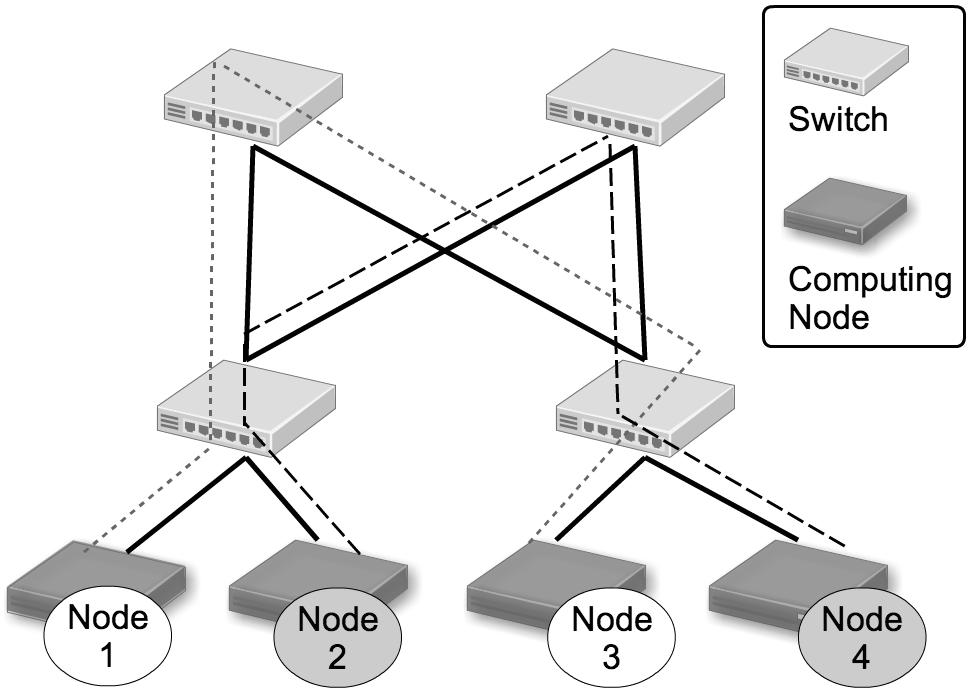
\includegraphics[width=.6\linewidth]{problem-routing1.png}
    \caption{Link Contention on Fat-tree}%
    \label{fig:problem-routing1}
\end{figure}

\begin{figure}
    \centering
    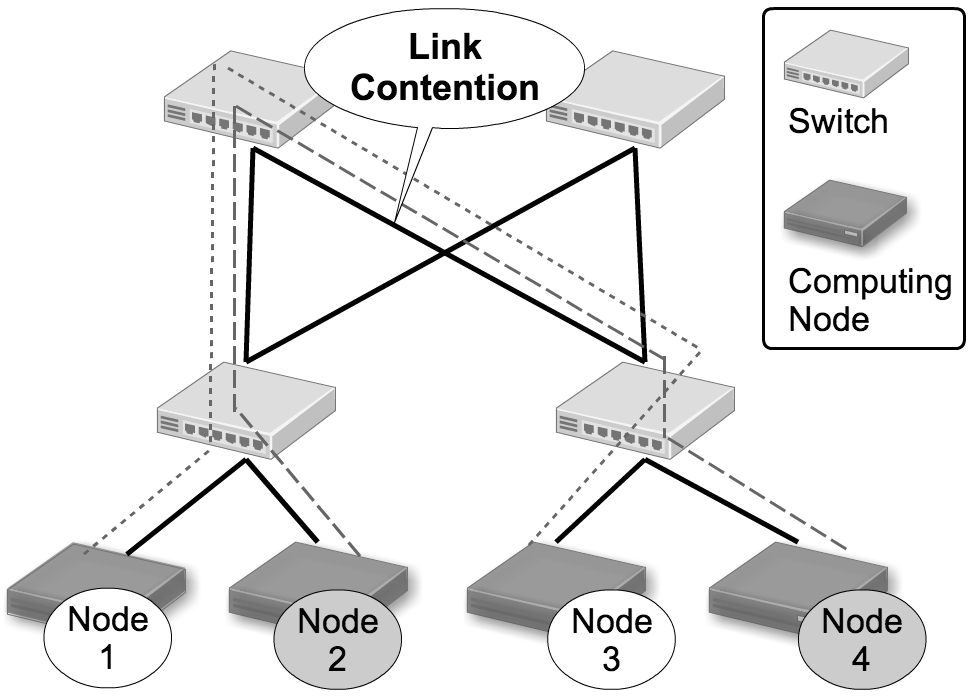
\includegraphics[width=.6\linewidth]{problem-routing2.png}
    \caption{Load Balancing Routes on Fat-tree}%
    \label{fig:problem-routing2}
\end{figure}

Various algorithms for balancing traffic in a network with redundant
routes have been proposed. Equal-Cost Multi-Path routing (ECMP)~\autocite{ecmp} is
a standardized load balancing strategy mainly used in L3 switches. For each
communication between two hosts, if multiple equal cost routes are available,
ECMP selects one route from among them. The decision of which route to use is
based on the header fields (\emph{e.g.} source and destination addresses) of
each packet. A hash function is applied to the header fields to generate the
corresponding hash value for the header fields, where every value in the hash
value space are evenly assigned to one of the equal cost routes.

InfiniBand~\autocite{infiniband} is a computer network communication link
commonly used in the area of HPC and a data center. InfiniBand supports
multiple routing methods. One of those methods is a min-hop routing
algorithm, which calculates the minimum hop route between every
computing node pair. If multiple minimum hop routes for a single
computing node pair are available, the algorithm assigns a route so that
usage among links is equalized.

The problem of these existing conventional load balancing mechanisms is
that they do not consider the characteristics of communication for MPI
applications. In general, MPI applications cannot retrieve usage
information of the underlying network or control it. MPI communication
does not occur evenly among computing nodes, and its sources and
destinations are biased. This may cause inequality of link usage that
decreases bandwidth between computing nodes. Ultimately, this decrease
of available bandwidth can lead to performance degradation of MPI
applications.

\subsection{Research Goals}

From our discussion above, we believe that an intelligent network control
mechanism which recognizes the communication pattern needed by MPI\_Allreduce
and effectively uses the bandwidth of each link by distributing the traffic
among redundant routes is essential. Therefore, in this research, we introduce
Software-Defined Networking (SDN) to enable such dynamic network control
dependent on the communication pattern of MPI applications.

We try to accelerate MPI\_Allreduce on a cluster system with a fat-tree
interconnect. This study integrates the dynamic network control ability of SDN
with MPI in order to avoid link contention and evaluates the performance of
MPI\_Allreduced based on our proposed mechanism.

\section{Proposal}\label{sec:iii-proposal}

In this section, we present our proposed mechanism for
MPI\_Allreduce. First, we briefly explain the architecture of
SDN, a core concept of our approach. After that, the proposed mechanism
is detailed. Lastly, the implementation of the proposed mechanism is
described.

\subsection{Proposed MPI\_Allreduce Using SDN}

\subsubsection{The Basic Idea Behind the Proposed Solution}

The basic idea behind the proposed solution is to improve the
inefficient communication in MPI in order to enhance the performance of
MPI applications. The fact that the MPI application cannot retrieve
usage information of the underlying network results in a potential
inefficiency in terms of communication. In this chapter, we focus on the
inequality of the link usage among the interconnect of a cluster system. Since
the bandwidth of links is limited, such inequality results in contention in
heavy traffic links.

In this chapter, we use redundant routes of the interconnect to ease the
inequality of link usage, based on an assumption that the cluster system has a
fat-tree interconnect. Through this traffic distribution, contention in the
links is expected to ease, which speeds up communication.

\subsubsection{Blueprint of Proposed SDN-enhanced MPI\_Allreduce}

The proposed mechanism is composed of three modules. These three modules are
the SDN controller, LLDP daemon and the SDN MPI\_Allreduce library. They are
deployed onto a cluster system as illustrated in
Fig.~\ref{fig:proposal-placement}. The SDN controller is deployed onto a
management node, which is a computer that is not involved in the actual
computation of the MPI application, but is used for controlling the whole
cluster system such as in deploying jobs to the system. LLDP daemon runs in
the background on all computing nodes. The SDN MPI\_Allreduce library is not a
stand-alone application, but a static library that must be linked to MPI
applications at compile time. Each computing node can run one or more MPI
processes, but in this chapter, we assume each computing node runs only one MPI
process.

\begin{figure}
    \centering
    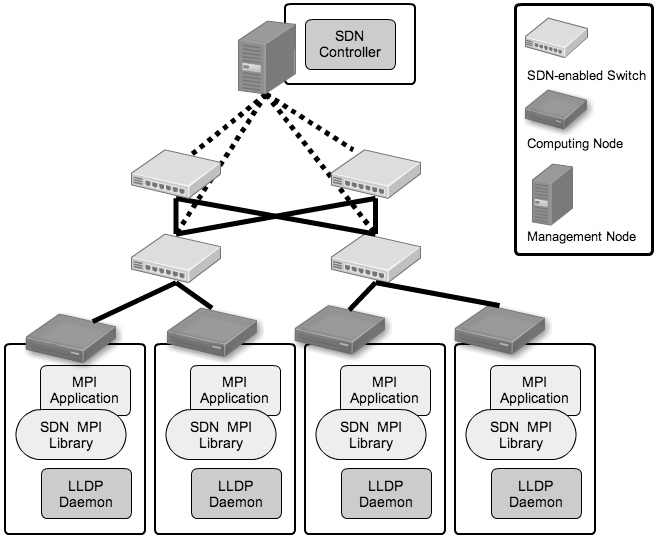
\includegraphics[width=.6\linewidth]{proposal-placement.png}
    \caption{Placement of the Modules Composing SDN-enhanced MPI\_Allreduce}%
    \label{fig:proposal-placement}
\end{figure}

The interaction among these modules is composed of two phases: the
initialization phase at the MPI application startup and the main phase at the
MPI\_Allreduce call. Figure~\ref{fig:proposal-sequence} is a UML sequence
diagram that illustrates how the modules cooperate with each other. MPI\_Init
is an MPI function that initializes the MPI execution environment, which must
be called on the application startup. After MPI\_Init finishes, all MPI
processes notify their own IP address and MPI \emph{rank} number to the SDN
controller. This information obtained from MPI processes are held by the
controller until the execution of the MPI application finishes.

\begin{figure}
    \centering
    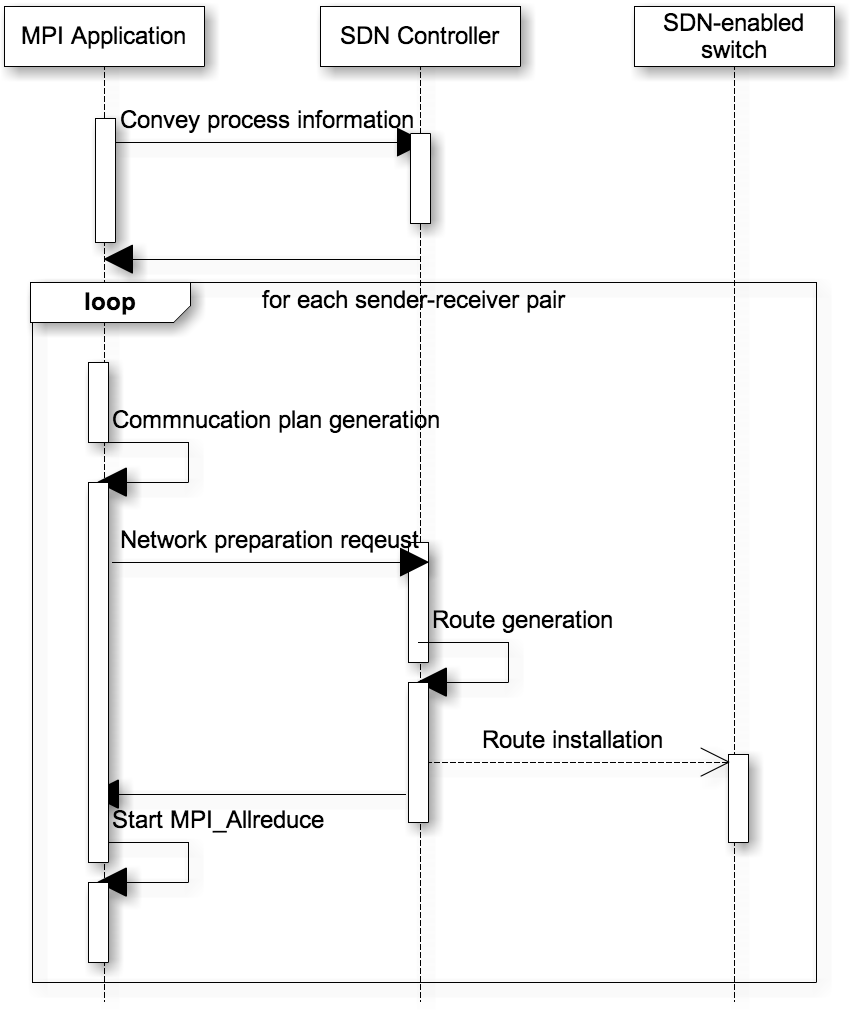
\includegraphics[width=.6\linewidth]{proposal-sequence.png}
    \caption{Sequence Diagram of Proposed Mechanism}%
    \label{fig:proposal-sequence}
\end{figure}

When MPI\_Allreduce is called, the rank 0 process generates the
\emph{communication plan} of MPI\_Allreduce. This communication plan is a set
of sender process and receiver process pairs during the MPI\_Allreduce
communication. After the communication plan generation, this set is sent to
the SDN controller by the rank 0 process. As soon as the SDN controller
receives the communication plan, it generates a route for each sender-receiver
pair. Subsequently, the SDN controller programs each SDN-enabled switch so
that the MPI packets are routed along the pre-generated route. After the
entire communication plan is processed, MPI\_Allreduce is called to start the
actual data transfer and calculation of the MPI\_Allreduce operation.

\subsection{Implementation of SDN MPI\_Allreduce}

To realize the proposed mechanism, we have developed three modules which
work as an integrated system. This section explains the detailed
implementation of these three modules.

\subsubsection{LLDP Daemon}

Each of the computing nodes runs a LLDP (Link Layer Discovery
Protocol)~\autocite{lldp} daemon in the background. This daemon is designed to
emit LLDP packets containing hardware information periodically, which are
received by the SDN-enabled switches and used for topology discovery. Some
LLDP daemon implementations~\autocite{lldpd,openlldpd} already exist. However we
have developed a new, minimal daemon to easily add and tweak features so that
it can cooperate with the other programs composing the whole system.

This daemon detects all available network interfaces installed on a
computer and queries its interface index, MAC address and IP address.
This information is packed into a single LLDP packet and sent out from
each network interface periodically. The interval is set to 1 second in
this prototypical implementation to speed up topology discovery.
However, it can be a longer period in practical systems so that its
topology does not change frequently.

As described above, the LLDP daemon emits a few hundred byte long
packets to the network every second. We consider this traffic is as
small enough so that it does not cause serious side effects on the
actual MPI process, for instance taking CPU time away from the
application or consuming too much bandwidth that could affect the MPI
communication. Generation of such LLDP packets is also not difficult
work for the computer, so we consider the impact to the application is
not severe.

\subsubsection{SDN Controller}

The SDN controller has four functionalities. The main feature of the SDN
controller is to prepare a route for MPI\_Allreduce that avoids
link contention and to install this routing to SDN-enabled switches. The
controller is also responsible for detecting the topology and use of the
interconnect, responding to Address Resolution Protocol (ARP) requests
from computing nodes and the routing of non-MPI traffic. This controller
is coded with the Trema framework~\autocite{trema}, a framework designed for
easily developing OpenFlow controllers in the Ruby~\autocite{ruby} language.

The first functionality is topology detection. How detection is
performed is as follows. The controller periodically requests every
switch to send out an LLDP packet from each of their physical ports.
This LLDP packet contains two kinds of information: datapath ID (a
number that uniquely distinguishes the switches) and port number (port
index where the packet is sent out). Moreover, all computing nodes also
emit LLDP packets from the LLDP daemon described above. The controller
is notified when a LLDP packet arrives at the controller. After that, it
parses the packet to obtain information on the packet's origin, to
examine whether the packet came from a computing node or an SDN-enabled
switch, and its MAC address/Datapath ID and Interface index/Port number.
Using this information from its neighbors, an adjacency list is
generated. From this adjacency list, a network topology graph is
constructed, which is used in the route generation and routing. If the
packet is from a computing node, the source MAC address and IP address
are registered in a MAC address - IP address table used in the ARP
responding functionality.

The second functionality is replying to ARP requests. An ARP request is
a L2 broadcast packet, so it causes a \emph{broadcast storm} problem
inside a network that contains a loop inside it. Since the target of
this chapter is a network that has redundant routes, it always has a loop
in it. Thus, the controller instructs the switches to reply to the
received ARP request, instead of the computing node that has the
corresponding IP address. The IP address that corresponds to the MAC
address is obtained from the MAC address - IP address table described
above.

The third functionality is route generation and installation for
MPI\_Allreduce communication. This functionality targets the flow of packets
pertaining to MPI\_Allreduce so that other MPI communication is not affected.
When the MPI application starts the proposed MPI\_Allreduce, the rank 0
process calculates the \emph{communication plan} of the MPI\_Allreduce.

The route searching algorithm used here for its speed and simplicity is
the \emph{Dijkstra} algorithm~\autocite{Dijkstra1959}. The Dijkstra
algorithm solves the shortest route problem for a graph with
non-negative link weights. In this proposed mechanism, link weights are
considered the number of total routes that go through that link. Under
this assumption, the shortest route means a route that shares links with
other routes. For each pair of sender processes and receiver processes,
a route is generated with the Dijkstra algorithm. After that, the weight
of all links contained in the generated route is incremented. This
procedure is repeated for all sender and receiver process pairs. This
algorithm selects the route that shares links with other routes from
multiple possible routes, which results in a distribution of routes.

Algorithm~\ref{lst:code-generate-route} is a pseudo-code for the algorithm.
First, an empty array \emph{routes} is initialized. After that, the
route search is performed for each sender-receiver pair. The resulting
route is added to \emph{routes} and the link weight (which is the number
of total routes that use that link) of each links is incremented. After
all routes have been generated, these routes are installed to the
SDN-enabled switches.

\begin{algorithm}
    \caption{Pseudocode of Route Generation.}%
    \label{lst:code-generate-route}
    \begin{algorithmic}
        \STATE routes = emptyArray();
        \STATE nodes = nodes in the topology graph;
        \STATE links = links in the topology graph;
        \FORALL{sender-receiver pair}
            \STATE route = dijkstra(nodes, links, sender, receiver);
            \STATE routes.push(route);
            \FORALL{link in route}
                \STATE link.weight += 1;
            \ENDFOR
        \ENDFOR
    \end{algorithmic}
\end{algorithm}

The fourth functionality is route generation and installation for
non-MPI traffic. For non-MPI traffic such as ICMP and SSH packets, the
SDN controller generates the minimum hop routes between computing nodes
and installs them on demand.

\subsubsection{SDN MPI\_Allreduce Library}

An MPI application that wants to use the proposed MPI\_Allreduce must be
linked with the SDN MPI\_Allreduce library. This library contains two
essential functions, SDN\_MPI\_Init and SDN\_MPI\_Allreduce. The application
is required to call SDN\_MPI\_Init on its launch, while SDN\_MPI\_Allreduce is
the SDN enhanced version that replaces the conventional MPI\_Allreduce.

SDN\_MPI\_Init opens a TCP connection with the SDN controller and notifies the
IP address and MPI rank number of the process that has called itself.
SDN\_MPI\_Allreduce generates the communication plan for the MPI application,
which is a set of sender process and receiver process pairs during the
communication in MPI\_Allreduce.

Several algorithms to realize the Allreduce operation have been proposed. This
chapter focuses on \emph{recursive doubling}~\autocite{Thakur2005}, since it
requires more inter-node communication compared with other algorithms, which
means more possibility of optimization in terms of communication.
Figure~\ref{fig:recursive-doubling} shows how the recursive doubling algorithm
works. In this context, the \emph{distance} between two MPI processes is
defined as the absolute value of the difference of rank numbers. In the first
step, processes that are 1 distance apart exchange their data and perform the
reduction operation between the data that the process has originally held and
with the just exchanged data. In the second step, processes that are 2
distance apart exchange their data, and in step \(p\), processes that are
\(2^{p - 1}\) distance apart exchange their data. The SDN MPI\_Allreduce
library memorizes all process pairs that have to communicate and exchange data
by following each step of the recursive doubling algorithm. For each of those
pairs, the library notifies the SDN controller to prepare each route.

\begin{figure}
    \centering
    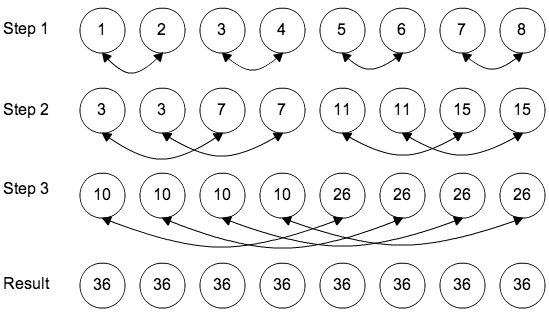
\includegraphics{recursive-doubling}
    \caption{Recursive Doubling Algorithm}%
    \label{fig:recursive-doubling}
\end{figure}

\section{Evaluation}\label{sec:iii-evaluation}

\subsection{Experimental Environment}

An experiment was conducted to compare the execution time of the
proposed MPI\_Allreduce and conventional
MPI\_Allreduce. The experimental environment is illustrated in
Fig.~\ref{fig:experiment-environment}. This experiment was performed on
a real cluster system consisting of 28 computing nodes and 6 SDN-enabled
switches, which forms a two-tier fat-tree topology. The computing nodes
and SDN-enabled switches were all connected with 1 Gigabit Ethernet
links, which compose a non-full bisection bandwidth network.

In addition to the network connecting the computing node and switches,
another network was prepared for control and management. This network
connects computing nodes, SDN-enables switches and the SDN controller.
The interaction between the SDN controller and SDN switches is performed
via OpenFlow protocol with this management network. The computing node
that runs MPI's rank 0 process and the SDN controller also communicates
with this network. Other computing nodes were connected to the
management network as well, but those connections were not used in this
experiment.

CentOS 6.4 was installed on all computers including the computing nodes and
SDN controller. The SDN controller was developed using a SDN controller
framework Trema~\autocite{trema} 0.4.6 and Ruby~\autocite{ruby} 1.9.3. The SDN
MPI\_Allreduce Library and the benchmark application were written in C and
compiled with gcc 4.4.7. As a representative of a conventional MPI,
Open MPI~\autocite{Gabriel2004} 1.5.4 was used.

\begin{figure}
    \centering
    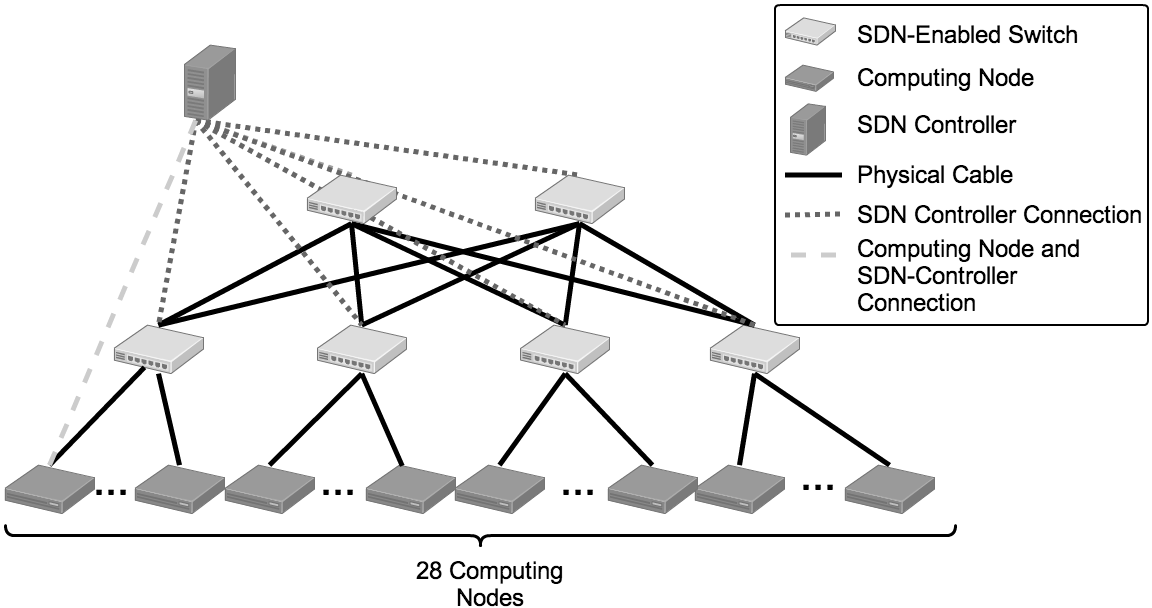
\includegraphics[width=.8\linewidth]{experiment-environment.png}
    \caption{Experimental Environment}%
    \label{fig:experiment-environment}
\end{figure}

\subsection{Measurement Result}

An MPI benchmark application that repeats MPI\_Allreduce 20
times and calculates the average execution time of the function was used
for comparing the execution time of the proposed MPI\_Allreduce
with its Open MPI counterpart.

Figure~\ref{fig:evaluation-8nodes} shows the measurement results using 8
nodes, where the horizontal axis indicates the message size and the
vertical axis shows the average time taken to execute
MPI\_Allreduce. The solid line and dashed line represent the
execution time of the proposed mechanism and Open MPI implementation,
respectively. Figure~\ref{fig:evaluation-8nodes-normalized} shows the
normalized performance improvement of the proposed mechanism in
comparison with the Open MPI implementation. The maximum of performance
improvement is 29\%.

\begin{figure}
    \centering
    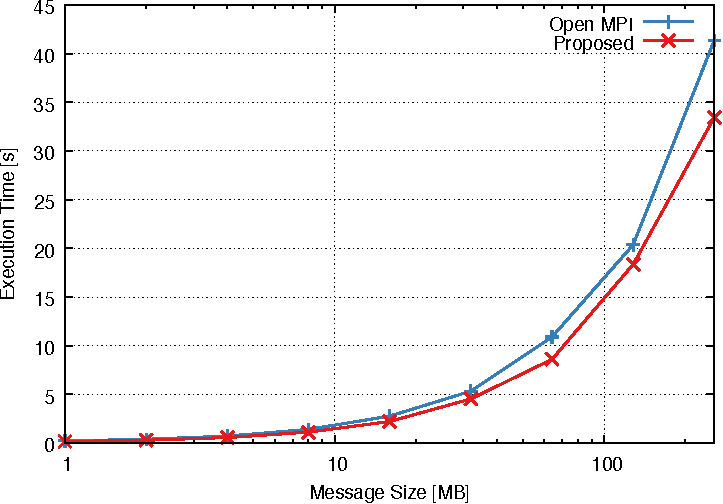
\includegraphics{allreduce_8nodes}
    \caption{Comparison of Execution Time of MPI\_Allreduce on 8 Computing Nodes}%
    \label{fig:evaluation-8nodes}
\end{figure}

\begin{figure}
    \centering
    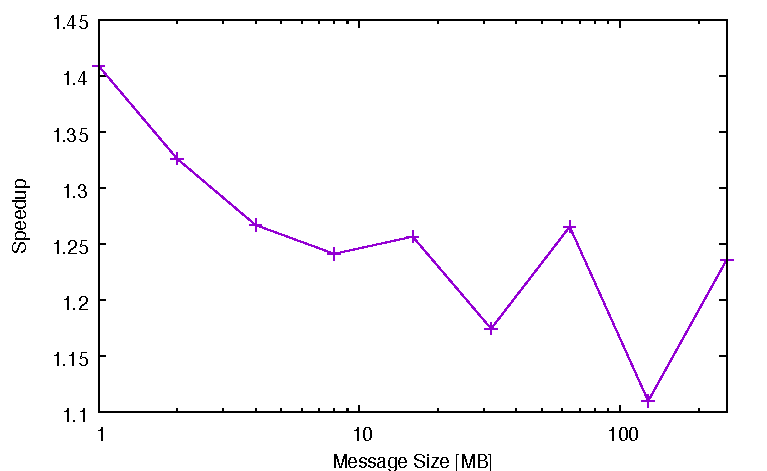
\includegraphics{allreduce_8nodes_speedup}
    \caption{Normalized Performance Improvement of Proposed MPI\_Allreduce on 8 Computing Nodes}%
    \label{fig:evaluation-8nodes-normalized}
\end{figure}

Figure~\ref{fig:evaluation-16nodes} shows the result of using 16 nodes.
Figure~\ref{fig:evaluation-16nodes-normalized} indicates the normalized
performance improvement of the proposed MPI\_Allreduce. It
shows how the proposed mechanism reduces the execution time of
MPI\_Allreduce for 36\% at most.

\begin{figure}
    \centering
    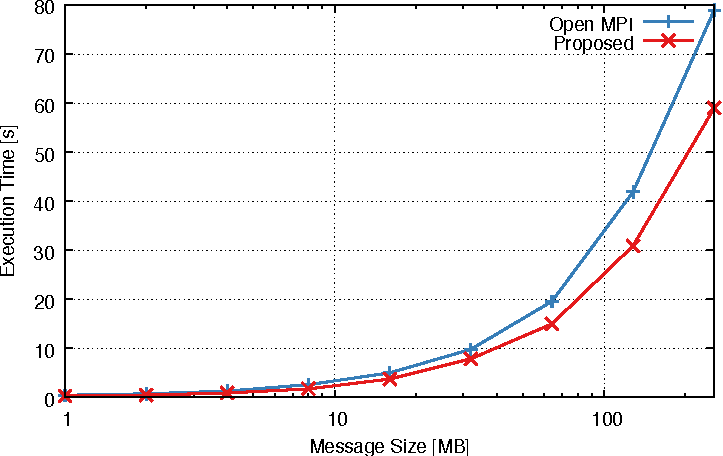
\includegraphics{allreduce_16nodes}
    \caption{Comparison of Execution Time of MPI\_Allreduce on 16 Computing Nodes}%
    \label{fig:evaluation-16nodes}
\end{figure}

\begin{figure}
    \centering
    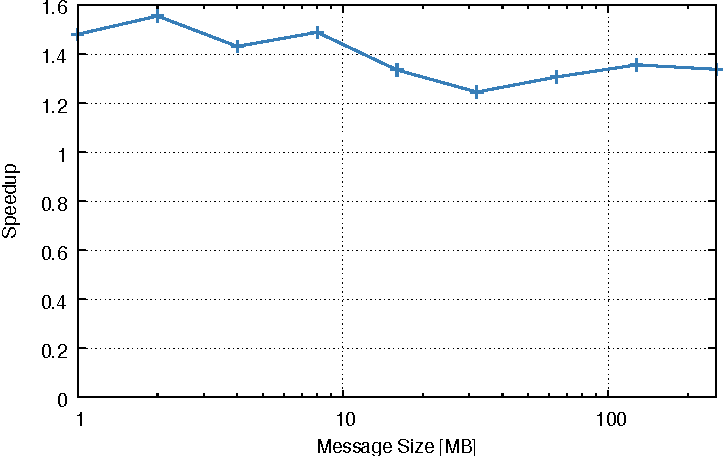
\includegraphics{allreduce_16nodes_speedup}
    \caption{Normalized Performance Improvement of Proposed MPI\_Allreduce on 16 Computing Nodes}%
    \label{fig:evaluation-16nodes-normalized}
\end{figure}

\section{Related Work}\label{sec:iii-related-work}

There have been many research works related to MPI\@. Since MPI is just a
specification for standard APIs for parallel programming, several algorithms
for collective operations have been proposed and implemented targeting several
network technology. As a representative example of such works,
MVAPICH~\autocite{mvapich} can be raised. MVAPICH is an MPI implementation
targeting InfiniBand, which most of high-performance computing systems ranked
in TOP500 has adopted. In literature~\autocite{PjesivacGrbovic2011}, Sur \emph{et
al.} designed MPI library by leveraging novel InfiniBand-offered features.
They explored new architectures from system point of view and new programming
paradigms from application point of view for keep scaling out applications on
more powerful computing systems. Literature~\autocite{Jiuxing2004} also
investigated MPI communication protocol focusing on RDMA operations in
InfiniBand. Our approach has some points in common in terms that our research
also aims to benefit from the features of the underlying network, while our
work differs from that we leverage Software Defined Networking instead of
InfiniBand from the purpose of investigating the feasibility of dynamic
control of network from application point of view.

Past works including existing MPI implementations have been successful
in switching between multiple algorithms depending on message size, node
number, \emph{etc.} to accelerate collective communication of MPI\@. Using
such a mechanism, estimation of the threshold value for parameters like
message size, node number, \emph{etc.} is essential. Pjesivac-Grbovic \emph{et
al.}~\autocite{PjesivacGrbovic} compared several parallel communication models
that are frequently used for dynamically estimating the threshold values. In
contrast, our current implementation always uses recursive doubling for
executing MPI\_Allreduce. Therefore, our system has a disadvantage in the
cases where small data size is treated on MPI\_Allreduce and thus the latency
is more respected than the bandwidth. For this disadvantage, we introduce
automatic algorithm switching leveraging estimation models mentioned in the
work of Pjesivac-Grbovic \emph{et al.}, depending on the situations.

The Fabric Collective Accelerator (FCA)~\autocite{fca} is a product by
Mellanox Technologies with the target of accelerating collective
communication on clusters with InfiniBand interconnect. FCA accelerates
collective communication by offloading computations to an InfiniBand
Host Channel Adapter (HCA). It also optimizes communication flow
according to job and topology. FCA optimizes collective tree and rank
placement to control communication flow. In contrast, our proposed
mechanism is capable of adaptively reconfiguring the network itself,
which is more flexible. FCA also requires InfiniBand hardware, but we
focus on a commodity Ethernet network.

Furthermore, there have been many research reports focusing on adaptive
use of networks for high-performance computing. Literature~\autocite{Geoffray2008}
proposed an adaptive routing method on Myrinet and the above mentioned
literature~\autocite{Jiuxing2004} explored the adaptive use of multiple
independent networks on InfiniBand. Our research also aims for a dynamic use
of the underlying interconnection network, but differs in that we attempted to
use a different interconnection network.

\section{Conclusion}\label{sec:iii-conclusion}

We have attempted to reduce the execution time of
MPI\_Allreduce by combining Software-Defined Networking (SDN)
with MPI\@. By using SDN, we have proposed a new network control mechanism
that can effectively make use of redundant routes by having SDN interact
with an MPI application communication pattern. We have designed and
implemented a system of three modules cooperating together to realize
our proposed mechanism. The evaluation showed that the proposed
MPI\_Allreduce decreased the execution time for 36\% at most
compared with a conventional implementation of MPI\_Allreduce.
As a result, we have confirmed the superiority of the proposed mechanism
over conventional methods.

Several issues to tackle have remained for the realization of practical
and useful MPI\_Allreduce leveraging SDN\@. The first issue to
achieve is the limitation of the number of nodes. As
MPI\_Allreduce has adopted recursive doubling algorithm. Under
our current implementation of the proposed MPI\_Allreduce, the
number of nodes is expected to be a power of 2, or \(2^p\). For scalable
and flexible use of MPI\_Allreduce, this limitation must be
solved.

In addition, on modern computing platforms where multiple cores exist in
a single computing node, the assumption set in this preliminary stage of
our research is neither practical nor realistic. Therefore, by
integrating kernel-assisted communication such as KNEM~\autocite{Goglin2013}
or CMA~\autocite{cma} with our proposed method, we need to consider
intra-node communication for pure MPI jobs. Also, computing paradigms
such as the hybrid use of OpenMP with MPI must be considered for
enhancing practicality. Also, other implementations of MPI such as
MVAPICH~\autocite{mvapich} are essential for investigating the practicality
and usefulness of SDN\@.

The second issue is the handling of the small data size.
MPI\_Allreduce happens in the small data size ranging from 8 to
32 bytes as well as in the larger data size in which we have focused.
When MPI\_Allreduce uses such a small data size, the latency is
more important than the bandwidth and this has been the initial focus of
our work. Under the current implementation of MPI\_Allreduce,
our MPI\_Allreduce would be problematic due to the incurred
overhead. Therefore, the introduction of automatic algorithm switching
leveraging estimation models summarized in Pjesivac-Grabovic et
al.,~\autocite{PjesivacGrbovic} may be explored after careful evaluation through
measurement experiments of MPI\_Allreduce for a small data size.

The third issue regards the necessity of additional experiments on a
larger scale environment. In this research, we have verified the
feasibility and possibility of the proposed MPI\_Allreduce
through the experiments using a simple prototypic implementation.
However, because OpenFlow switches are expensive and thus only a small
size cluster is available for our research group, we could only conduct
a small number of experiments in a small cluster environment. Therefore,
after succeeding with a more sophisticated implementation of the
proposed MPI\_Allreduce, we understand that further experiments
on a larger scale environment are essential for the evaluation of
scalability.

Since our current implementation requires communication between MPI
processes and SDN controller and route generation for each MPI
communication request, the SDN controller might be a bottleneck on
larger environments. Therefore, we are planning to cache IP addresses
and MPI rank numbers for each process in the SDN controller.
Furthermore, we enhance our implementation so that only the root process
interacts with the SDN controller and conveys information of all
participating processes in the collective communication.
